\documentclass[12pt,a4paper]{article}
\usepackage[UTF8]{ctex}
\usepackage{amsmath,amssymb}
\usepackage{booktabs}
\usepackage{siunitx}
\usepackage{float}
\usepackage{fancyhdr}   % 页眉页脚控制
\usepackage{geometry}
\usepackage{subfigure}  % 子图排版
\usepackage{subcaption}
\usepackage{graphicx}
\usepackage{listings} % 代码排版宏包
\usepackage{xcolor} % 代码高亮颜色
\usepackage{enumitem} % 列表格式控制宏包
\geometry{left=2.5cm,right=2.5cm,top=2.5cm,bottom=2.5cm}

\pagestyle{fancy}
\fancyhf{} % 清空默认页眉页脚
\fancyhead[L]{\small 牛顿环}       % 左上角页眉
\fancyhead[R]{\small 2513318}          % 右上角章节名
\fancyfoot[C]{\thepage}                   % 居中页码（页脚）
\renewcommand{\headrulewidth}{0.4pt}      % 页眉线粗细
\renewcommand{\footrulewidth}{0.4pt}      % 页脚线粗细
%报告开始
\begin{document}
	%设置课程标题
	\begin{center}
		\heiti\LARGE{《大学基础物理实验》课程实验报告}
	\end{center}
	%设置实验人信息以及实验时间表格
	\begin{center}
		\begin{tabular}{lcr}
			{\songti 姓名及学号：陈秋实2513318}  \quad 专业：密码科学与技术 \quad 组别：L组1号 \\
			{\songti  学院：密码与网络空间安全学院 \quad 实验时间：2026年5月29日~星期五~下午}\\
		\end{tabular}
	\end{center}
	\vspace{-0.2cm}
	{\noindent}	 \rule[-10pt]{16cm}{0.05em}\\
	\vspace{-0.4cm}
	%实验题目
	\begin{center}
		\LARGE\textbf{牛顿环}
	\end{center}


	\section{实验目的}
	\par 1.观察等厚干涉现象，并利用等厚干涉测量凸透镜表面的曲率半径。
	\par 2.了解读数显微镜的使用方法。

	\section{实验器材}
	\par 牛顿环装置，钠灯，读数显微镜

	\section{实验原理}
	\subsubsection*{牛顿环原理}
	\begin{figure}[!htbp]
		\centering
		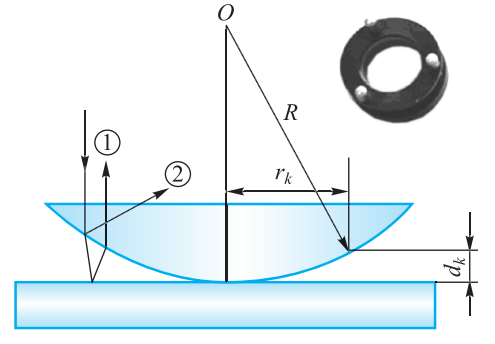
\includegraphics[width=0.5\textwidth]{牛顿环.png}
		\caption{牛顿环原理}
	\end{figure}
	\subsubsection*{测量原理}
	\par 在图1中，$R$为待测透镜凸面的曲率半径，$r_k$是第k级干涉环的半径，$d_k$是第k级干涉环所对应的空气间隙的厚度。如果入射光的波长为$\lambda$，则第k级干涉环所对应的光程差为
	\[
	\Delta_k = 2d_k+\frac{\lambda}{2}
	\]
	\clearpage
	\par 其中,$\dfrac{\lambda}{2}$为光由光疏介质入射到光密介质时，反射光的半波损失。因此，在接触点处($d_0$=0)的光程差为
	\[
	\Delta_0 = \frac{\lambda}{2}
	\]
	\par 在理想情况下，牛顿环的中心是一个几何暗点。但在实际情况中，透镜和平板玻璃接触时，由于有重力和压力存在，透镜的凸面和平板玻璃均发生形变，两者的接触不再是点接触，而是面接触。因此，牛顿环的零级暗条纹不是个点，而是一个较大的暗斑。
	\par 第$k$级干涉暗环处的光程差为
	\[
	\Delta_k = 2d_k+\frac{\lambda}{2} = (k+\frac{1}{2})\lambda
	\]
	\par 所对应的空气间隙的厚度为
	\[
	d_k = k\frac{\lambda}{2}
	\]
	\par 由于$R\gg d_k$,所以有
	\[
	r_k^2 = R^2-(R-d_k)^2 \approx 2Rd_x
	\]
	\par 可知第$k$级别的干涉暗环的半径为
	\[
	r_k = \sqrt{k\lambda R}
	\]
	\par 但是在实际测量中，无法确定干涉环圆心的位置，但是可以获得弦长
	\[
	l_k^2 = 4(r_k^2-s^2)
	\]
	\par 代入之前的公式，得到
	\[
	l_k^2 = 4k\lambda R-4s^2
	\]
	\par 为了得到斜率求出$R$,测量不同数据利用最小二乘法计算出斜率。

	\section{实验步骤}
	\par \textbf{一、点亮钠灯}\quad 几分钟后它将发出明亮的黄光。调节半透半反镜的倾角和左右方向，使显微镜的视场达到最亮。
	\par \textbf{二、找到暗纹}\quad 调节目镜，使得能够清晰的看清叉丝，将物镜的位置移动到最低，眼睛看着目镜，从下网上移动目镜，知道能够看清条纹，最后根据条纹的方向将叉丝移动到最中心的暗环处
	\clearpage
	\begin{figure}[!htbp]
		\centering
		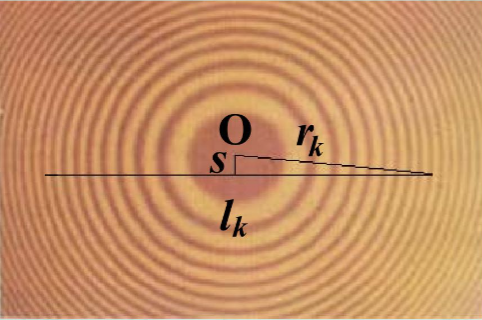
\includegraphics[width=0.5\textwidth]{牛顿环1.png}
		\caption*{牛顿环图片}
	\end{figure}

	\par \textbf{三、测量}\quad 通过旋钮移动叉丝的位置，测量不同级次的干涉环的弦长，\textbf{注意:}在实验过程中，为了避免回程差，需从45级次开始，一直向同一个方向进行测量。

	\section{数据处理}
	\begin{tabular}{|c|c|c|c|c|c|c|c|c|}
		\hline
		干涉级数 & 10 & 15 & 20 & 25 & 30 & 35 & 40 & 45 \\
		\hline
		干涉位置 (左)$\mathrm{mm}$ & 23.739 & 24.282 & 24.730 & 25.138 & 25.501 & 25.830 & 26.142 & 26.442 \\
		\hline
		干涉位置 (右)$\mathrm{mm}$ & 18.692 & 18.171 & 17.714 & 17.331 & 16.964 & 16.620 & 16.302 & 16.008 \\
		\hline
		弦长$\mathrm{mm}$ & 5.047 & 6.111 & 7.016 & 7.807 & 8.537 & 9.210 & 9.840 & 10.434 \\
		\hline
		弦长平方$\mathrm{mm}^2$ & 25.473 & 37.344 & 49.225 & 60.949 & 72.880 & 84.784 & 96.826 & 108.869 \\
		\hline
	\end{tabular}

	\subsubsection*{数据处理说明}
	\par 根据最小二乘法原理，对干涉级数 $k$ 与弦长平方 $l^2$ 进行线性拟合。设拟合直线方程为 $l^2 = a + bk$，其中 $b = 4\lambda R$ 为待求斜率。
	\par 首先计算各变量的平均值：
	\[
	\bar{k} = \frac{1}{8}\sum_{i=1}^{8}k_i = 27.5,\quad
	\overline{l^2} = \frac{1}{8}\sum_{i=1}^{8}l_i^2 = 67.04375
	\]
	\par 为便于计算回归系数，列出以下中间计算量(见表1)：

	\begin{table}[!htbp]
		\centering
		\begin{tabular}{|c|c|c|c|c|c|}
			\hline
			$k$ & $l^2$ & $k-\bar{k}$ & $l^2-\overline{l^2}$ & $(k-\bar{k})^2$ & $(k-\bar{k})(l^2-\overline{l^2})$ \\
			\hline
			10 & 25.473  & $-17.5$ & $-41.5708$ & 306.25  & 727.4881 \\
			\hline
			15 & 37.344  & $-12.5$ & $-29.6998$ & 156.25  & 371.2469 \\
			\hline
			20 & 49.225  & $-7.5$  & $-17.8188$ & 56.25   & 133.6406 \\
			\hline
			25 & 60.949  & $-2.5$  & $-6.0948$  & 6.25    & 15.2369 \\
			\hline
			30 & 72.880  & $2.5$   & $5.8363$   & 6.25    & 14.5906 \\
			\hline
			35 & 84.784  & $7.5$   & $17.7403$  & 56.25   & 133.0519 \\
			\hline
			40 & 96.826  & $12.5$  & $29.7823$  & 156.25  & 372.2781 \\
			\hline
			45 & 108.869 & $17.5$  & $41.8253$  & 306.25  & 731.9419 \\
			\hline
			\multicolumn{2}{|c|}{$\sum$} & — & — & 1050.00 & 2499.475 \\
			\hline
		\end{tabular}
		\caption{最小二乘法中间计算量}
	\end{table}

	\par 由表中求和结果可得：
	\[
	\sum(k-\bar{k})^2 = 1050.00,\quad \sum(k-\bar{k})(l^2-\overline{l^2}) = 2499.475
	\]
	\par 代入最小二乘法公式，得斜率：
	\[
	b = \frac{\sum(k-\bar{k})(l^2-\overline{l^2})}{\sum(k-\bar{k})^2} = \frac{2499.475}{1050.00} = 2.3805
	\]
	\par 截距：
	\[
	a = \overline{l^2} - b\bar{k} = 67.04375 - 2.3805 \times 27.5 = 1.5800
	\]
	\par 故拟合直线方程为：$l^2 = 1.5800 + 2.3805k$。
	代入$\lambda=589.3\mathrm{nm}$,解得$R=1009.864\ \mathrm{mm}$
	\par 相关系数 $R²=0.999985$
	\begin{figure}[!htbp]
		\centering
		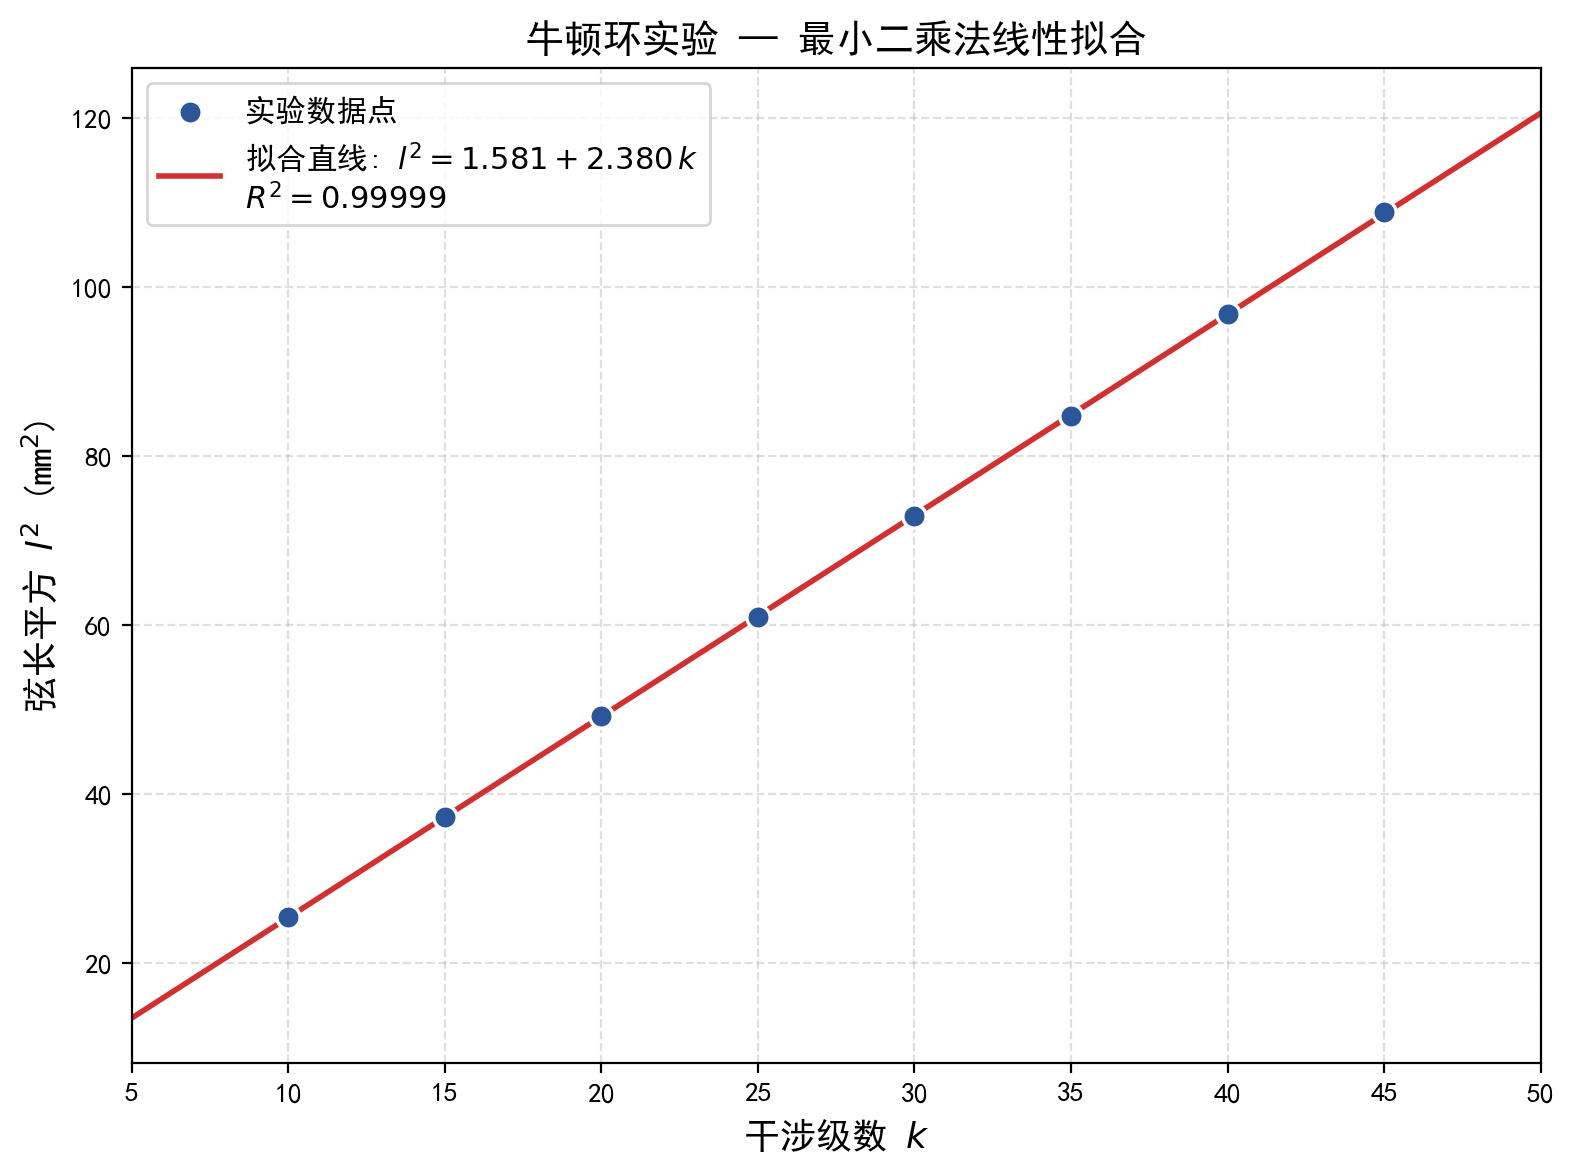
\includegraphics[width=0.8\textwidth]{least_squares_fit.png}
		\caption{数据拟合}
	\end{figure}



	\section{思考题}
	\subsubsection*{第一题}
	\par 因为不能保证叉丝移动轨迹刚好经过圆心，所以只能通过弦长的公式来计算。
	\subsubsection*{第二题}
	\par 先往一个方向移动超过需要测量的距离更多的距离，这样子再往回移动的过程中就可以先移动一段距离然后再测量，可以避免回空差。
	\subsubsection*{第三题}
	\par 1. 低级次条纹容易受到牛顿环装置接触面的灰尘、形变等影响，往往不呈比较理想的圆环形。
	\par 2. 低级次条纹比较粗不利于准确测量
	\par 3. 此外，由于牛顿环装置接触面的灰尘、形变等影响，低级次的条纹往往会混杂在一起，造成分辨不清，难以计数。
	\subsubsection*{第四题}
	\par 便于观察牛顿环现象且易于测量.如果视场过暗，则会导致无法看清干涉条纹，测量就会出现错误
	\subsubsection*{第五题}
	\par 1.测量时应先数45级次，然后从45级次开始测量，按级次从大到小再变大测量.测量时鼓轮必须朝一个方向转动：
	\par 2.45到10级次记录暗环外圈数值，10到45级次记录内圈数值，这样就能得到相对准确的弦长值。
\end{document}